\documentclass[a4paper,12pt]{article}
\usepackage{graphicx}% Required for inserting images
\usepackage{float}
\usepackage[hidelinks]{hyperref} 
\begin{document}
\date{}

\begin{titlepage}
    \centering
    \vspace*{1cm}

    
\includegraphics[width=0.4\textwidth]{images/UC_logo.png}\par\vspace{1cm}

    {\Huge\bfseries Machine Learning 2025/2026\par}
    \vspace{1.5cm}
    {\Large\itshape Detecting breast cancer from blood samples \\[1.5cm]}
{\Large \textnormal{Intermediate Report}}
\vfill
\vfill

        \begin{center}
            \large
            \textbf{Members: \\}
            Mariana Duarte, 2022212961\\
            Miguel Castela, 2022212972\\
            
    \end{center}
    
    \vfill
    
    {October, 2025 \par}
\end{titlepage}

%índice
\tableofcontents       
\newpage

\section{Introduction}

<<<<<<< HEAD
In this report we explain the implementation of a Machine Learning model capable of accurately identifying individuals diagnosed with breast cancer based on a blood sample dataset.

\noindent
The dataset used in this study consists of data from 116 patients, including 64 diagnosed with breast cancer and 52 belonging to a healthy control group. The nine analyzed variables comprise parameters such as age, body mass index (BMI), glucose and insulin concentrations, the HOMA index, the levels of leptin, adiponectin, resistin, and MCP-1.

=======
This work aims to develop a Machine Learning model capable of accurately identifying individuals diagnosed with breast cancer based on blood sample data.

The dataset used in this study consists of data from 116 patients, including 64 diagnosed with breast cancer and 52 belonging to a healthy control group. The nine analyzed variables comprise demographic and biochemical parameters, namely age, body mass index (BMI), glucose and insulin concentrations, the HOMA index, and the levels of leptin, adiponectin, resistin, and MCP-1.
>>>>>>> parent of b00b1e1 (commit final meta1)

\section{Methods and Methodologies}


\subsection{Data Partitioning}

<<<<<<< HEAD
The data was initially divided into three subsets: a training set (70\%), a test set (15\%), and a validation set (15\%). However, the test and validation sets were later merged, because during the first stage of the project there is no hyperparameter tuning, invalidating the need of a separate test and validation set. The classifiers were trained using the training set, while the test set is reserved for evaluating the classifiers’ performance and generalization ability. This was done using a stratified split, ensuring that the proportion of classes (\textit{Healthy} and \textit{Cancer}) was maintained in both subsets. \\
\noindent
After the partitioning, the data was normalized according to $\frac{x - \mu}{\sigma}$, so that each feature had a mean of 0 and a standard deviation of 1, ensuring comparability across variables with different value scales.
=======
The data were initially split into two subsets: a training set (70\%) and a test set (30\%). This split allows the model to be trained using only the training set, while the test set is reserved for evaluating the classifiers’ performance and generalization ability. The partitioning was performed in a stratified manner, ensuring that the proportion of classes (\textit{Healthy} and \textit{Cancer}) was maintained in both subsets. The data were normalized according to $\frac{x - \mu}{\sigma}$, so that each feature had a mean of 0 and a standard deviation of 1, ensuring comparability across variables with different scales.
>>>>>>> parent of b00b1e1 (commit final meta1)

\subsection{Feature Selection}

<<<<<<< HEAD
Before applying the classifiers, it is necessary to evaluate the discriminative power of the original variables to identify those most relevant for distinguishing between the two classes. Firstly, we plot box/violing plots for each feature to see which are more discriminative. After, these were ranked and picked based on various feature selection methods
=======
Before applying the classifiers, it is necessary to evaluate the discriminative power of the original variables to identify those most relevant for distinguishing between classes and reducing redundancies.  
This step aims to improve model performance and reduce the dimensionality of the data.
>>>>>>> parent of b00b1e1 (commit final meta1)

\subsubsection{Kruskal-Wallis Test}

The Kruskal-Wallis test is a non-parametric statistical test used to compare two or more independent samples.  
In this context, it was applied to assess the statistical relevance of each variable in distinguishing between the \textit{Healthy} and \textit{Cancer} classes.  
The function \texttt{stats.kruskal} from the \texttt{scipy} library was used to compute the p-value for each feature.

The null hypothesis (\(H_0\)) assumes that the distributions of samples from different classes come from the same population, i.e., that the variable has no discriminative power.  
When the p-value is below 0.05, \(H_0\) is rejected, concluding that the samples come from distinct populations and that the feature has discriminative ability.

\subsubsection{ROC Curve and AUC}
\label{sec:ROC}

The ROC (Receiver Operating Characteristic) method is particularly suitable for binary classification problems.  
The ROC curve represents the true positive rate (TPR) as a function of the false positive rate (FPR) for different decision thresholds.  
The area under the curve (AUC) provides a quantitative measure of classifier performance.

An AUC value of 1 indicates perfect separation between classes, while a value of 0.5 indicates performance equivalent to random guessing.  
Thus, ROC/AUC analysis allows identifying variables with the highest discriminative capacity.

\subsubsection{Correlation Matrix}

The correlation matrix is used to assess linear relationships between variables.  
High correlations indicate redundancy, i.e., two features vary similarly.  
Analyzing this matrix helps select subsets of less correlated variables, reducing redundancy and improving classifier efficiency.

<<<<<<< HEAD
The correlation matrix of the nine features was computed to assess the degree of linear dependence between variables.  
This analysis was implemented using the \texttt{numpy.corrcoef} function and visualized with \texttt{Plotly Express} as a heatmap.  


\subsection{Feature Reduction}

=======
>>>>>>> parent of b00b1e1 (commit final meta1)
\subsubsection{Principal Component Analysis (PCA)}

PCA is an unsupervised a dimensionality reduction technique that projects data onto a new set of orthogonal axes, called principal components (PCs), which maximize data variance.  
The goal is to find a reduced set of variables capturing most of the information contained in the original data with minimal variance loss.

Eigenvectors define the direction (axis orientation), while eigenvalues represent the variance explained along those directions.

Three criteria were used to determine the optimal number of components to retain:

\begin{itemize}
    \item \textbf{95\% Threshold:} select components that collectively explain at least 95\% of the total variance;
    \item \textbf{Scree Criterion:} identify the point where the eigenvalue plot (scree plot) stabilizes, indicating components with marginal contribution;
    \item \textbf{Kaiser Criterion:} retain only components with eigenvalues greater than 1 (applicable to normalized data).
\end{itemize}

\subsubsection{Linear Discriminant Analysis (LDA)}
<<<<<<< HEAD
\noindent
LDA aims to project data into a lower-dimensional subspace that maximizes class separability while minimizing within-class variability.  
This supervised method finds a direction (or several) that maximizes the ratio between between-class variance and within-class variance, according to Fisher's criterion.
\noindent
Since the number of discriminant directions that can be found is limited by the number of classes, LDA reduces the data dimensionality to at most \textit{(number of classes $-$ 1)}.
\noindent
The result is a linear combination of the original variables, usable for both visualization and classification.
\noindent
The \texttt{LinearDiscriminantAnalysis} class from \texttt{scikit-learn} was then fitted to the dataset to compute the optimal discriminant direction that maximizes class separation.
\noindent
The data were projected onto the first linear discriminant (LDA1), and the resulting one-dimensional representation was visualized using a scatter plot, allowing a qualitative evaluation of the separation between healthy and cancer samples.
=======
>>>>>>> parent of b00b1e1 (commit final meta1)

Linear Discriminant Analysis aims to project data into a lower-dimensional subspace that maximizes class separability while minimizing within-class variability.  
The method finds a direction (or several) that maximizes the ratio between between-class variance and within-class variance, according to Fisher's criterion.

The result is a linear combination of the original variables, usable for both visualization and classification.

\subsection{Classifiers}

After feature selection and reduction, three distance-based classifiers were applied:

\subsubsection{Euclidean Distance Classifier}

In this classifier, each unknown sample is assigned to the class whose mean is closest in terms of Euclidean distance, defined as:

\[
||x - m||_e = \sqrt{\sum_{i=1}^{d} (x_i - m_i)^2}
\]

where \(x\) represents the sample and \(m\) the class mean.  
This method assumes that all variables have equal weight and similar variance.

\subsubsection{Mahalanobis Distance Classifier}

The Mahalanobis distance is a more sophisticated metric that accounts for correlations among variables and differences in scale.  
It is defined as:

\[
||x - y||_m = \sqrt{(\mathbf{x} - \mathbf{y})^{T} \mathbf{C}^{-1} (\mathbf{x} - \mathbf{y})}
\]

where \(\mathbf{C}\) is the covariance matrix of the variables.  
This classifier adapts to the true geometry of the data, being more robust when variables are correlated.

\subsubsection{Fisher LDA Classifier}

The Fisher LDA classifier combines linear discriminant analysis with the Mahalanobis metric.  
It determines a weight vector \(\mathbf{w}\) that maximizes class separation and defines a decision threshold.  
Decisions are based on the sign of the linear discriminant:

\[
y = \mathbf{w}^T \mathbf{x} + b
\]

where \(b\) is the bias term.  
This classifier is particularly effective for two-class problems and when distributions are approximately Gaussian.
<<<<<<< HEAD
\noindent
To implement the Fisher LDA classifier, several computational steps were followed. The mean vector of each class was then computed to represent its centroid in the multidimensional feature space. 
Subsequently, the within-class scatter matrices were calculated for both classes, quantifying the covariance of samples around their respective means. 
These matrices were summed to obtain the total within-class scatter matrix ($S_w$).

The optimal discriminant direction was determined by multiplying the inverse of this matrix with the difference between the class mean vectors, according to:

\[
\mathbf{w} = S_w^{-1}(\boldsymbol{\mu}_{\text{Cancer}} - \boldsymbol{\mu}_{\text{Healthy}})
\]

A bias term ($b$) was then computed to position the decision boundary approximately midway between the two class means, given by:

\[
b = -\frac{1}{2}\mathbf{w}^T(\boldsymbol{\mu}_{\text{Cancer}} + \boldsymbol{\mu}_{\text{Healthy}})
\]
Finally, the classifier’s performance was evaluated using standard metrics, including 
accuracy, sensitivity, specificity, precision, and F1-score, providing a quantitative assessment of its discriminative ability.



\subsection{Experimental Setup}

The \textit{main} script implements the complete data analysis and classification workflow. The dataset partitions are loaded and perform the feature selection and reduction tasks on the training split. Finally, multiple classifiers are fitted using the training data (all features, top 5 ranked using kruskall-wallis and ROC-AUC, PCAs, and LDA). These were tested for accuracy with the test split. In the euclidean distance classifier this is done by computing the mean feature vectors of the Healthy and Cancer classes from the training data and assigning each test sample to the class whose mean is closest in Euclidean distance. The Mahalanobis classifier extends this by considering feature correlations through the covariance matrix computed from the training data, allowing it to capture the underlying data structure more accurately when classifying unseen testing samples. Similarly, Fisher’s Linear Discriminant classifier determines the optimal projection axis that maximizes class separability based solely on the training set, and then applies this learned transformation to the testing samples to evaluate how well the model generalizes to new data. Additionally to the sensitivity, specificity, precision, F1-score, and accuracy metrics used to evaluate each classifier's performance on the test samples, a ROC-AUC score was calculated using the same methods employed in the feature extraction tests (True Positive Rate and False Positive Rate using \texttt{roc\_curve} from \texttt{scipy}).  
This metric provides an aggregate measure of each classifier’s discriminative ability across all decision thresholds, offering a more comprehensive evaluation of the overall performance.\\

\noindent
To ensure the robustness and reliability of the results, each experiment was executed five times using different random seeds.
For every run, the dataset was divided into random training and testing subsets using a stratified split, ensuring that the class proportions (Healthy and Cancer) were preserved across all partitions.
After completing the five runs, the performance metrics score were averaged to obtain stable and representative results, minimizing the influence of random initialization and data partitioning variability.

=======
>>>>>>> parent of b00b1e1 (commit final meta1)

\section{Result Analysis}

<<<<<<< HEAD
The following section presents the analysis of the obtained results, focusing on the performance of the implemented classifiers and dimensionality reduction methods.

\noindent
Figure \ref{fig:violin} illustrates the distribution of the extracted features for both Healthy and Cancer samples using violin plots. This visualization provides a detailed view of the data dispersion and density for each feature, highlighting differences in their statistical distributions between the two classes. The width of each violin indicates the probability density of the data at different values, allowing a direct comparison of variability and central tendency across features.

\begin{figure}[H] 
    \centering
    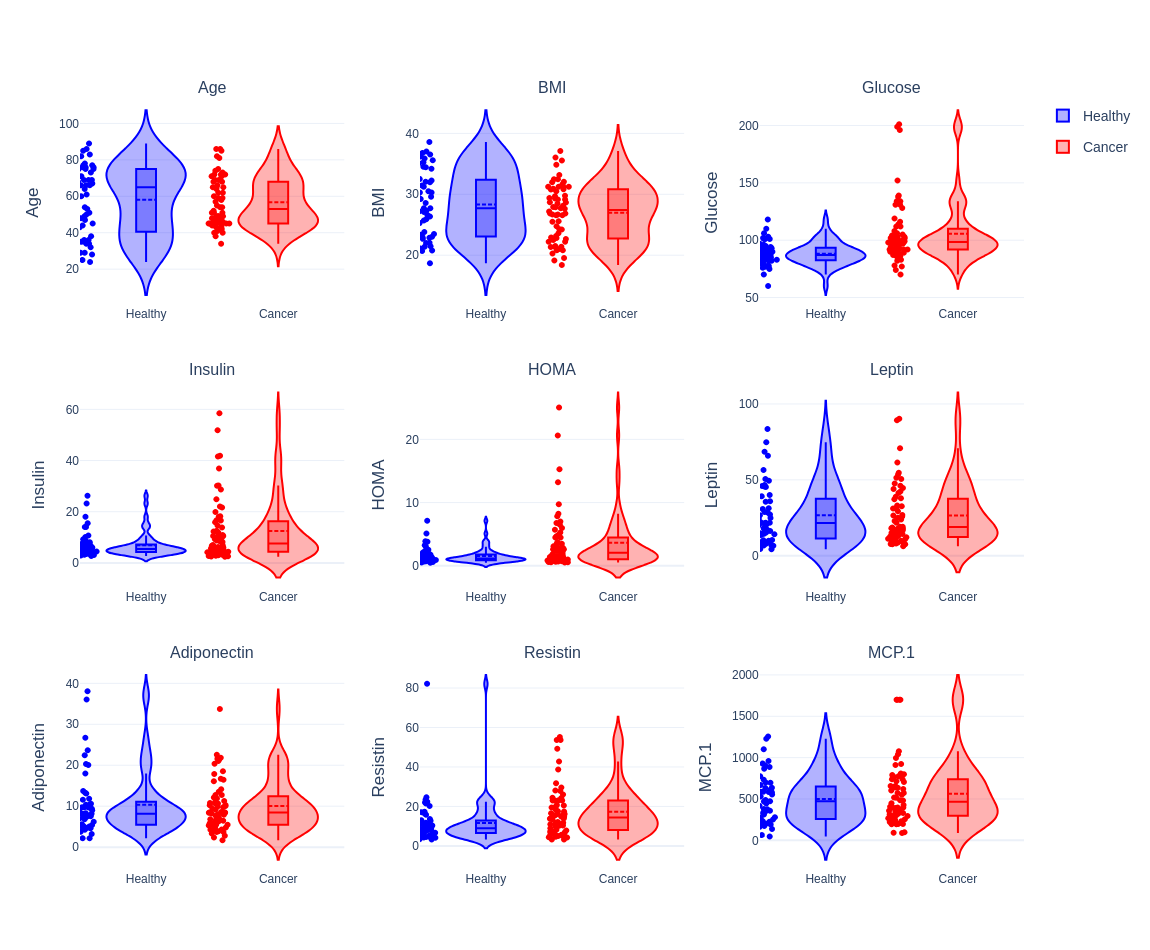
\includegraphics[width=1.1\textwidth]{images/violin.png}
    \caption{Violin plots.}
    \label{fig:violin}
\end{figure}
\noindent
The subplots clearly point towards some features being more discriminative than others. Glucose, HOMA, resistin and Insulin have much higher differences in their value ranges than the others, more overlapping features. These observations are confirmed when doing the feature selection and dimensionality reduction.

\noindent
To compare the performance of the classifiers, the performance metrics were first calculated using all features without any preprocessing. The results are presented in the table below.

\begin{table}[H]
\centering
\caption{Classifier results using all the features.} 
\begin{tabular}{lccc}
\hline
\textbf{Metric} & \textbf{Euclidean} & \textbf{Mahalanobis} & \textbf{Fisher LDA}  \\
\hline
Sensitivity (\%) & 50.5 & 65.3 & 63.2 \\
Specificity (\%) & 80.0 & 82.5 & 82.5 \\
Precision (\%) & 75.3 & 82.0 & 81.3 \\
F1-score (\%) & 60.3 & 72.2 & 70.6 \\
Accuracy (\%) & 64.0 & 73.1 & 72.0 \\
ROC-AUC (\%) & 73.8 & 79.5 & 79.2 \\
\hline
\end{tabular}
\label{tab:allfeatures_classifiers}
\end{table}

\noindent
Analyzing Table \ref{tab:allfeatures_classifiers}, it is evident that some metrics, such as sensitivity, F1-score, and accuracy, fall below desired levels.

\noindent
The ROC curves were plotted, and the AUC values were calculated for each feature, as shown in the figure below.

\begin{figure}[H] 
    \centering
    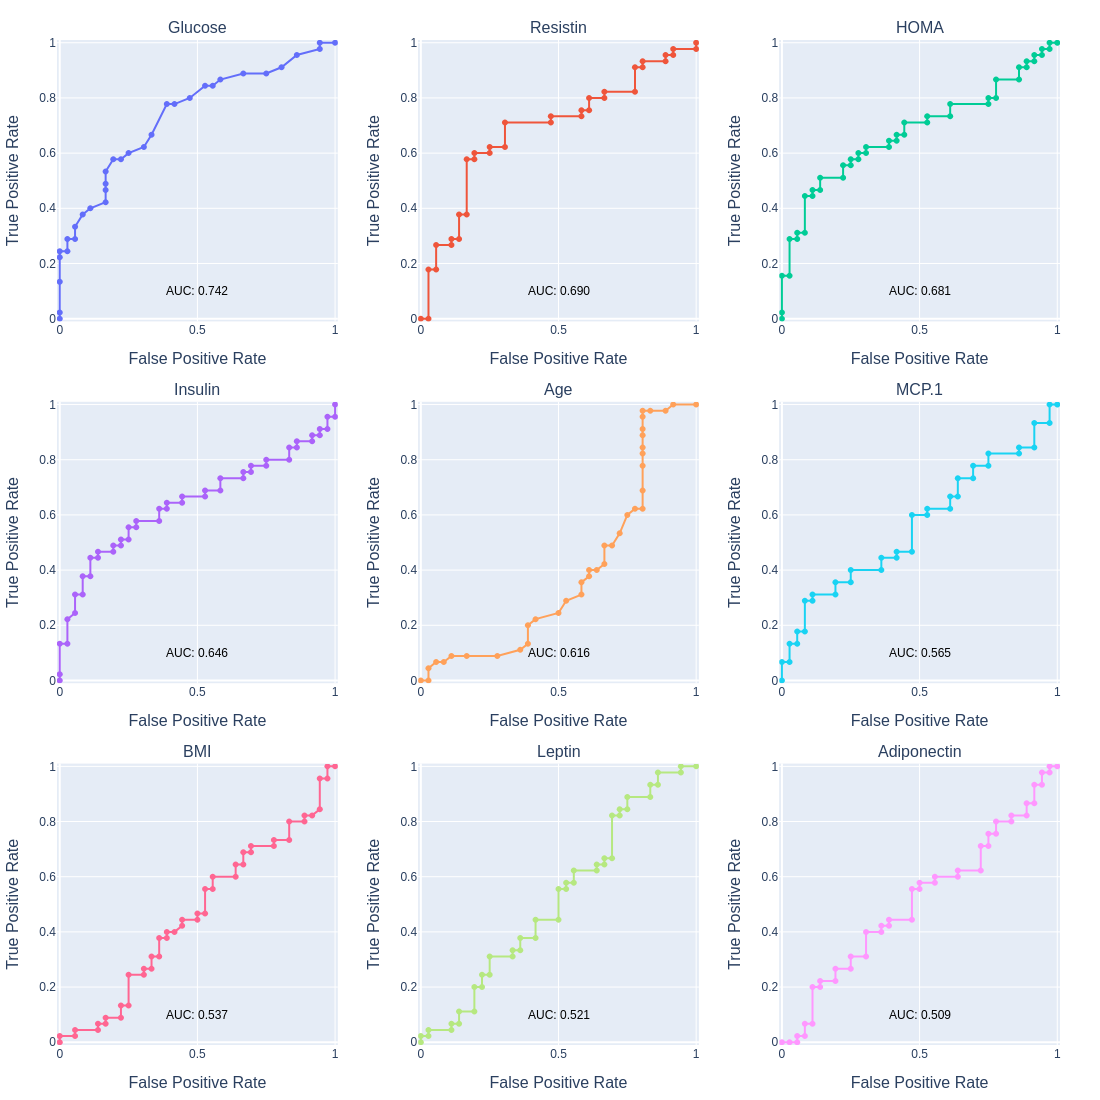
\includegraphics[width=1.1\textwidth]{images/ROC_AUC.png}
=======
As curcas ROC foram traçadas e foram calculadas as AUC para cada feature, como se mostra na imagem abaixo.

\begin{figure}[H] 
    \centering
    \includegraphics[width=1.1\textwidth]{roc.png}
>>>>>>> parent of b00b1e1 (commit final meta1)
    \caption{ROC curves for different feature sets.}
    \label{fig:roc_curves}
\end{figure}

<<<<<<< HEAD
\noindent
According to Figure \ref{fig:roc_curves}, the AUC values of all features were ranked in order to identify the top five features to be used in the training of the classifiers.

\begin{table}[H]
\centering
\caption{Median ROC-AUC values across runs (sorted).} 
\begin{tabular}{lc}
\hline
\textbf{Feature} & \textbf{AUC} \\
\hline
Glucose & 0.7540 \\
HOMA & 0.6753 \\
Resistin & 0.6580 \\
Insulin & 0.6287 \\
BMI & 0.6148 \\
Age & 0.5438 \\
MCP.1 & 0.5309 \\
Leptin & 0.5302 \\
Adiponectin & 0.5302 \\
\hline
\end{tabular}
\label{tab:AUC values}
\end{table}
\noindent
According to the Table \ref{tab:AUC values}, we can conclude that the top five features are Glucose, HOMA, Resistin, Insulin and BMI.
 
\noindent
The different classifiers were applied using these features, and the resulting performance metrics for the test data are presented in the table below.
=======
 Tal como mencionado em \ref{sec:ROC}, as features cuja AUC é menor que 0.5 não são úteis, pelo que, como se pode ver na figura \ref{fig:roc_curves}, as top 5 features selecionadas por este método são: METER AS FEATURES.
 
Desta forma aplicaram-se os diferentes classificadores a este método, obtendo-se os resultados das métricas presentes na tabela abaixo para os dados de teste.
>>>>>>> parent of b00b1e1 (commit final meta1)

\begin{table}[H]
\centering
\caption{Classifier results using the top 5 features (ROC selection).} 
\begin{tabular}{lccc}
\hline
\textbf{Metric} & \textbf{Euclidean} & \textbf{Mahalanobis} & \textbf{Fisher LDA} \\
\hline
<<<<<<< HEAD
Sensitivity (\%) & 52.6 & 63.2 & 62.1 \\
Specificity (\%) & 81.2 & 75.0 & 75.0 \\
Precision (\%) & 77.1 & 74.7 & 74.3 \\
F1-score (\%) & 62.5 & 68.2 & 67.4 \\
Accuracy (\%) & 65.7 & 68.6 & 68.0 \\
ROC-AUC (\%) & 76.2 & 77.6 & 77.0 \\
=======
Sensitivity (\%) & 47.37 & 52.63 & 52.63 \\
Specificity (\%) & 75.00 & 68.75 & 68.75 \\
Precision (\%) & 69.23 & 66.67 & 66.67 \\
F1-score (\%) & 56.25 & 58.82 & 58.82 \\
Accuracy (\%) & 60.00 & 60.00 & 60.00 \\
>>>>>>> parent of b00b1e1 (commit final meta1)
\hline
\end{tabular}
\label{tab:roc_classifiers}
\end{table}

<<<<<<< HEAD
\noindent
According to Table \ref{tab:roc_classifiers}, the three classifiers yield similar values for each metric and occasionally show improvements compared to the results obtained using all features. However, this is not consistently observed.

\noindent
We generated the correlation matrix to analyze how the features in training vary with respect to each other. This is to determine whether they are highly or weakly correlated and to assess potential redundancy among them.
 
\begin{figure}[H] 
    \centering
    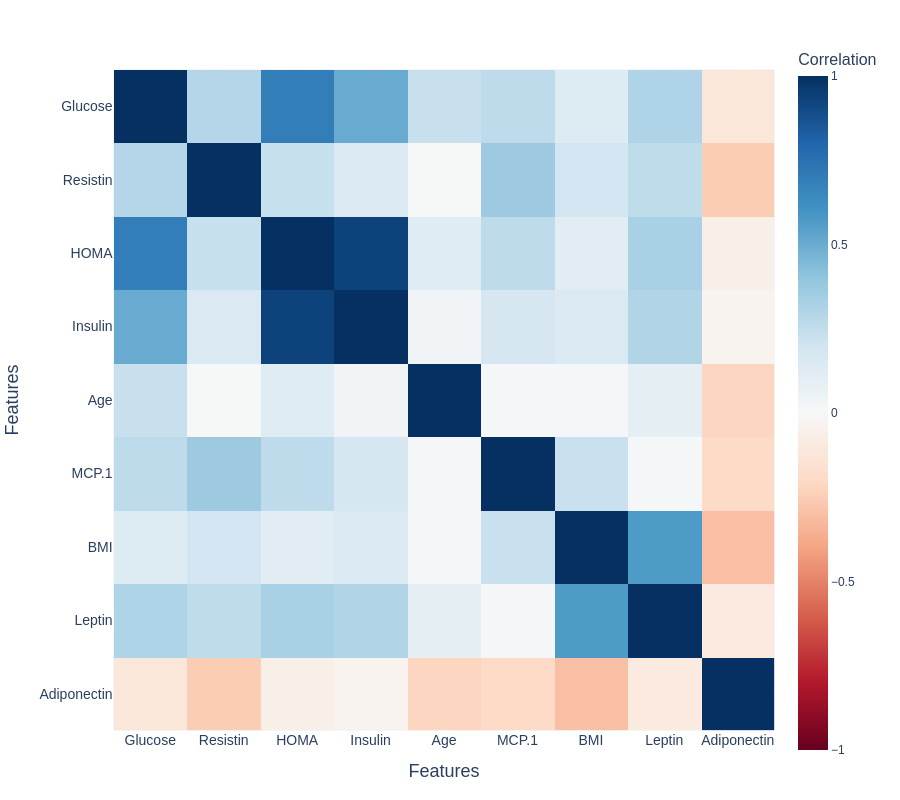
\includegraphics[width=1\textwidth]{images/CORRELATION_MATRIX.png}
=======
De acordo com a Tabela \ref{tab:roc_classifiers}, verifica-se que os três classificadores dão o mesmo valor de 60\% para a accuracy e que os restantes valores não se distanciam muito, como seria de esperar, uma vez que é tudo projetado a uma dimensão. Verifica-se ainda que o classificador Mahalanobis e Fisher LDA apresentam valores iguais para todas as métricas.

Fizemos a matriz de correlação para perceber como as features variam entre si, ou seja, se estão muito ou pouco correlacionadas para percebermos se são redundantes, isto é, explicam o mesmo.
 
\begin{figure}[H] 
    \centering
    \includegraphics[width=1.1\textwidth]{matriz_corr.png}
>>>>>>> parent of b00b1e1 (commit final meta1)
    \caption{Correlation matrix between features.}
    \label{fig:mcorr}
\end{figure}
\noindent
From Figure \ref{fig:mcorr}, we can observe that Adiponectin is the most weakly correlated with the other features, followed by Age and BMI.

<<<<<<< HEAD
\noindent
Next, we applied the Kruskal–Wallis test to rank the top five features by their H value. This indicates the degree to which each feature significantly differentiates between the groups, with higher H values reflecting stronger discriminatory power and greater relevance for distinguishing class differences.

\begin{table}[H]
\centering
\caption{Median Kruskal-Wallis H-statistic values across runs (sorted).} 
\begin{tabular}{lc}
\hline
\textbf{Feature} & \textbf{H} \\
\hline
Glucose & 15.3190 \\
HOMA & 7.2860 \\
Resistin & 5.9201 \\
Insulin & 3.9271 \\
BMI & 3.1253 \\
Age & 0.4558 \\
MCP.1 & 0.2259 \\
Adiponectin & 0.2169 \\
Leptin & 0.2169 \\
\hline
\end{tabular}
\label{tab:kruskal_h_values}
\end{table}

\noindent
From Table \ref{tab:kruskal_h_values}, we can identify the top five features as Glucose, HOMA, Resistin, Insulin and BMI, these were used on the classifiers.

\noindent
The performance metrics on the test data for the classifiers applied to the feature selection using the Kruskal–Wallis test are presented in the table below.
=======
Atraves da Figura \ref{fig:mcorr} verificamos que Adiponectin é muito pouco correlacionada com as outras features, assim como Age, MCP-1, VER MEHOR NO GRÁFICO QUE A FIGURA É MUITO PEQUENA    
Depois usámos o teste de Kruskal-Wallis para reduzir a dimensionalidade e obtermos o top 5 das features, cujo p-value é maior (ou menor?) que 0.05, o que indica que as amostras pertencem à mesma população. SE CALHAR FAZER TABELA COM OS VALORES DE P?
>>>>>>> parent of b00b1e1 (commit final meta1)

Os resultados das métricas aos dados de teste da aplicação dos classificadores à seleção das features com Kruskal-Wallis estão indicados na tabela abaixo.
\begin{table}[H]
\centering
\caption{Classifier results using the top 5 features (Kruskal-Wallis selection).}
\begin{tabular}{lccc}
\hline
\textbf{Metric} & \textbf{Euclidean} & \textbf{Mahalanobis} & \textbf{Fisher LDA} \\
\hline
<<<<<<< HEAD
Sensitivity (\%) & 52.6 & 63.2 & 62.1 \\
Specificity (\%) & 81.2 & 75.0 & 75.0 \\
Precision (\%) & 77.1 & 74.7 & 74.3 \\
F1-score (\%) & 62.5 & 68.2 & 67.4 \\
Accuracy (\%) & 65.7 & 68.6 & 68.0 \\
ROC-AUC (\%) & 76.2 & 77.6 & 77.0 \\
=======
Sensitivity (\%) & 47.37 & 52.63 & 52.63 \\
Specificity (\%) & 75.00 & 68.75 & 68.75 \\
Precision (\%) & 69.23 & 66.67 & 66.67 \\
F1-score (\%) & 56.25 & 58.82 & 58.82 \\
Accuracy (\%) & 60.00 & 60.00 & 60.00 \\
>>>>>>> parent of b00b1e1 (commit final meta1)
\hline
\end{tabular}
\label{tab:kruskal_classifiers}
\end{table}

<<<<<<< HEAD
\noindent
As can be seen in Table \ref{tab:kruskal_classifiers}, the results are identical to those obtained using the ROC-AUC curves. This identical performance of the classifiers can be explained by the fact that both approaches identified the same five features. This demonstrates that, for this dataset, both feature selection methods successfully capture the features with the strongest class-discriminative power.


\noindent
To analyze the principal components, the three methods described in Section \ref{sec:PCA} were applied.
\noindent
The variance explained by each principal component is shown in the figure below.

\begin{figure}[H] 
    \centering
    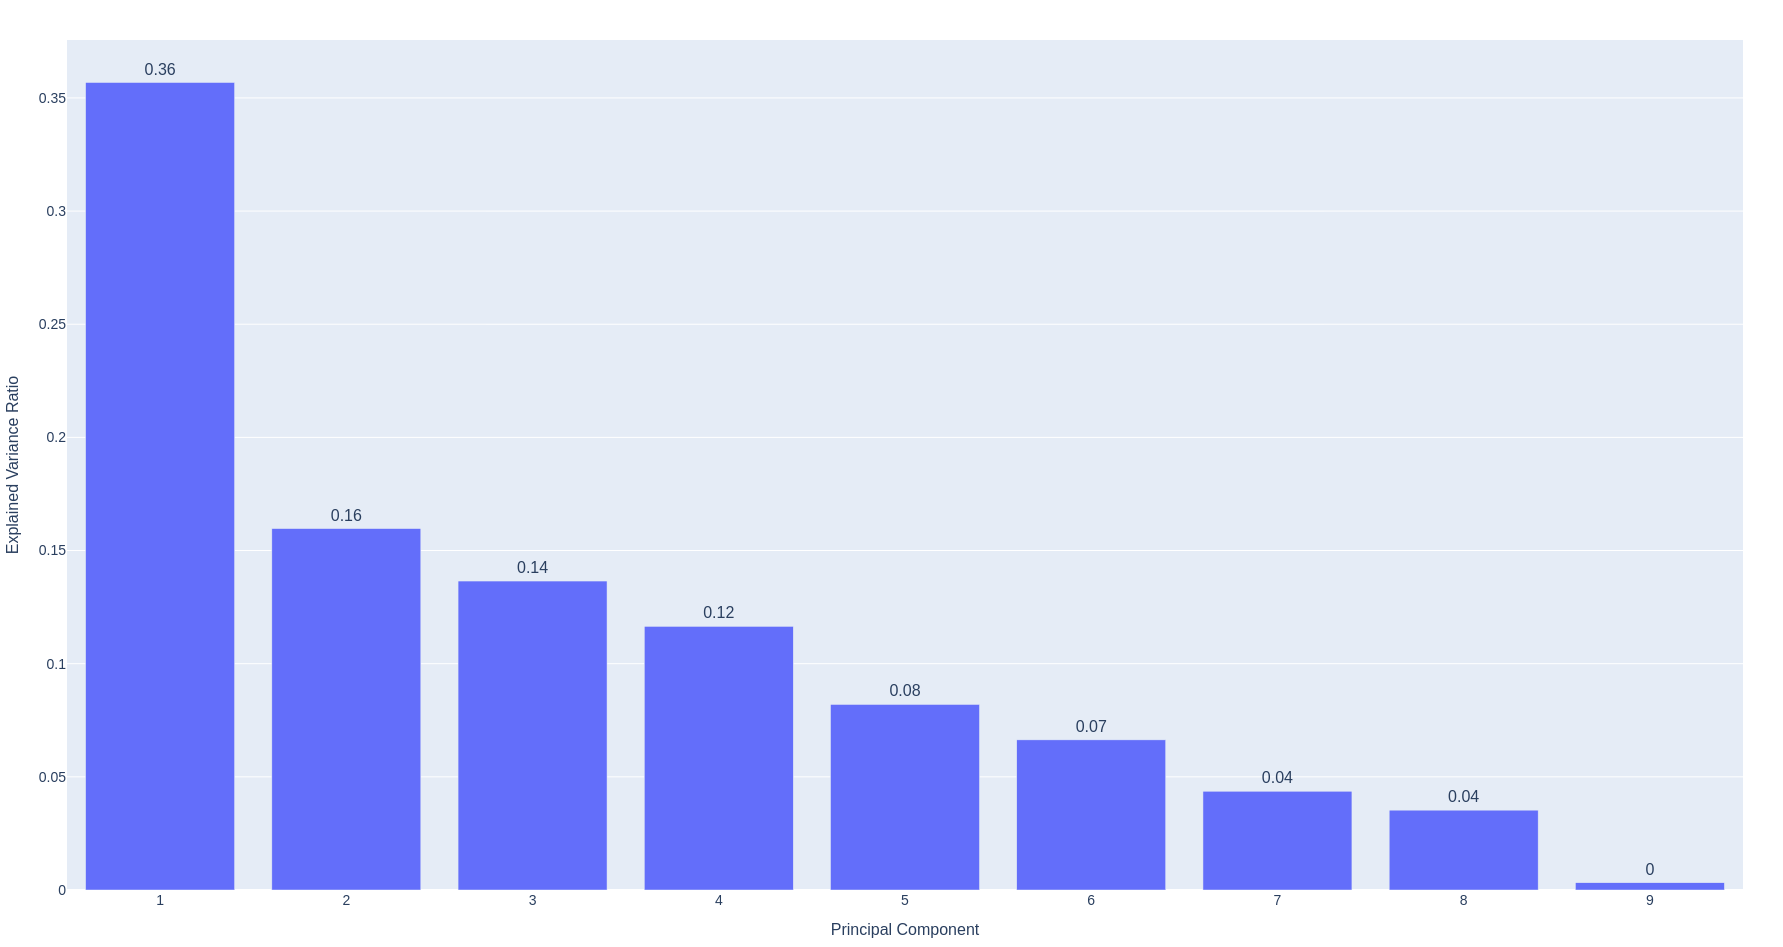
\includegraphics[width=1.1\textwidth]{images/PC_variance.png}
    \caption{Explained variance for each principal component.}
    \label{fig:PC_variance}
\end{figure}
\noindent
The 95\% criterion indicated that the first seven principal components are required to retain most of the information and preserve the highest variance in the data.
\noindent
To visualize the selection of PCs according to the Kaiser criterion and the Scree test, the corresponding plot is shown below.


\begin{figure}[H] 
    \centering
    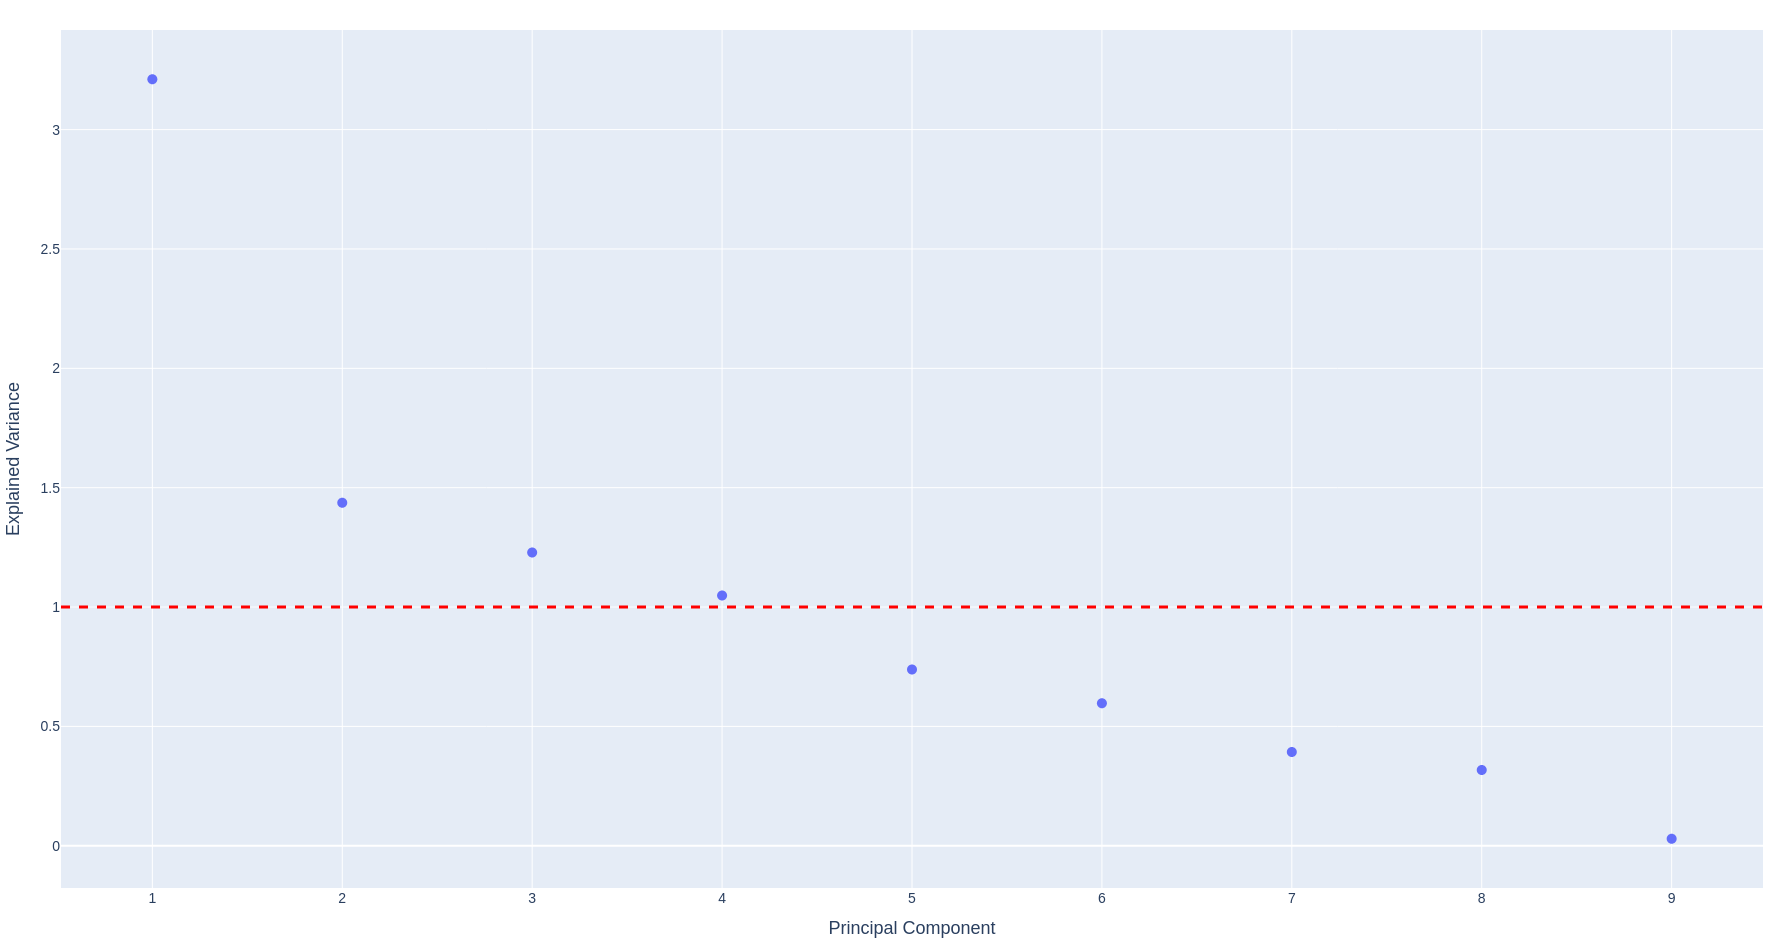
\includegraphics[width=1.1\textwidth]{images/PCA_Kaiser_Scree.png}
    \caption{Principal components projected in a Kaiser and Scree plot.}
    \label{fig:Kaiser_Scree}
\end{figure}

\noindent
By observing Figure \ref{fig:Kaiser_Scree}, it can be seen that, according to the Kaiser criterion, only the first four principal components are selected. In contrast, the Scree method does not allow for a clear conclusion, as no leveling-off of the curve of the eigenvalues is observed.
\noindent
The first principal component, which accounts for the largest variance, is shown in the figure below.

\begin{figure}[H] 
    \centering
    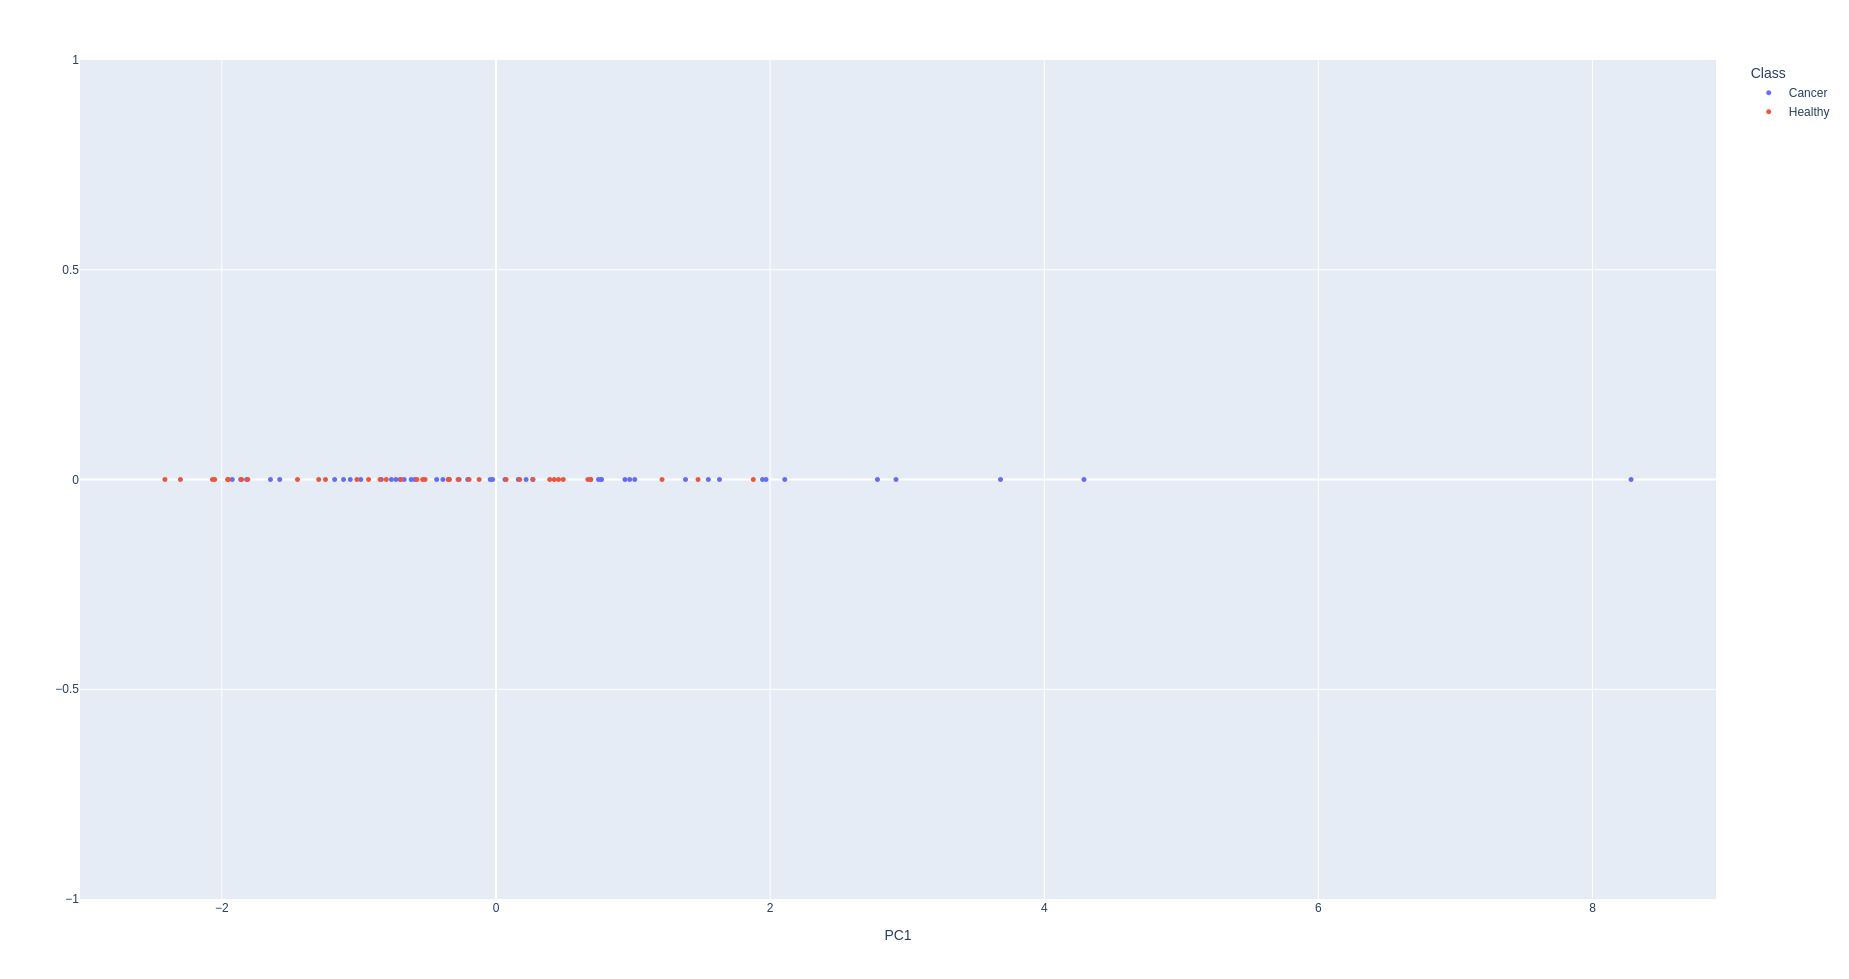
\includegraphics[width=1.1\textwidth]{images/PC1.png}
    \caption{First principal component.}
    \label{fig:pc1}
\end{figure}

\noindent
Among the three criteria used for PCA, the 95\% variance threshold provided the best results, as it retained 7 components while preserving most of the information.
The Scree criterion, on the other hand, suggested retaining only 4 components, which would likely result in a loss of information since the cumulative explained variance only reached a median of 78\%, this is possibly due to not having a clear PC among the top 5 that explains most of the variance.

Because of this we applied the 7 components that explain 95\% of the variance to our result analysis.
\noindent
Using the different classifiers on the testing data, the performance metrics were applied for this method, as presented in the table below.

=======
Como podemos observar através da Tabela \ref{tab:kruskal_classifiers}, os resultados são iguais aos obtidos para a curva roc pois selecioanram as mesmas features, como seria de esperar (ENCONTRAR MAIS JUSTIFICAÇÃO PARA OS RESULTADOS DAREM EXTAMENTE IGUAIS)


Depois através do PCA fomos ver quais eram as PC que apresentavam mais wejfiowjfiwkjo

\begin{figure}[H] 
    \centering
    
\includegraphics[width=1.1\textwidth]{PC1.png}
    \caption{PC1}
    \label{fig:pc1}
\end{figure}

>>>>>>> parent of b00b1e1 (commit final meta1)
\begin{table}[H]
\centering
\caption{Classifier results using the top 7 principal components from PCA.}
\begin{tabular}{lccc}
\hline
\textbf{Metric} & \textbf{Euclidean} & \textbf{Mahalanobis} & \textbf{Fisher LDA} \\
\hline
<<<<<<< HEAD
Sensitivity (\%) & 50.5 & 66.3 & 66.3 \\
Specificity (\%) & 80.0 & 80.0 & 80.0 \\
Precision (\%) & 76.0 & 80.2 & 80.2 \\
F1-score (\%) & 60.3 & 72.2 & 72.2 \\
Accuracy (\%) & 64.0 & 72.6 & 72.6 \\
ROC-AUC (\%) & 73.6 & 75.9 & 75.7 \\
=======
Sensitivity (\%) & 42.11 & 57.89 & 52.63 \\
Specificity (\%) & 81.25 & 62.50 & 62.50 \\
Precision (\%) & 72.73 & 64.71 & 62.50 \\
F1-score (\%) & 53.33 & 61.11 & 57.14 \\
Accuracy (\%) & 60.00 & 60.00 & 57.14 \\
>>>>>>> parent of b00b1e1 (commit final meta1)
\hline
\end{tabular}
\label{tab:pca_classifiers}
\end{table}

<<<<<<< HEAD
\noindent
According to Table \ref{tab:pca_classifiers}, it can be observed that the results obtained with the Mahalanobis and Fisher LDA classifiers are identical, as explained in Section \ref{sec:mahalanobis_fisher}. Nevertheless, some metrics, such as accuracy, F1-score, sensitivity, precision, and specificity, show slight improvements compared to the results obtained using all features or the top features selected via ROC-AUC and Kruskal-Wallis. However, these improvements are only observed when using the Mahalanobis and Fisher LDA classifiers.
\noindent
With LDA, the data was reduced to a single dimension, as shown in the figure below.

\begin{figure}[H] 
    \centering
    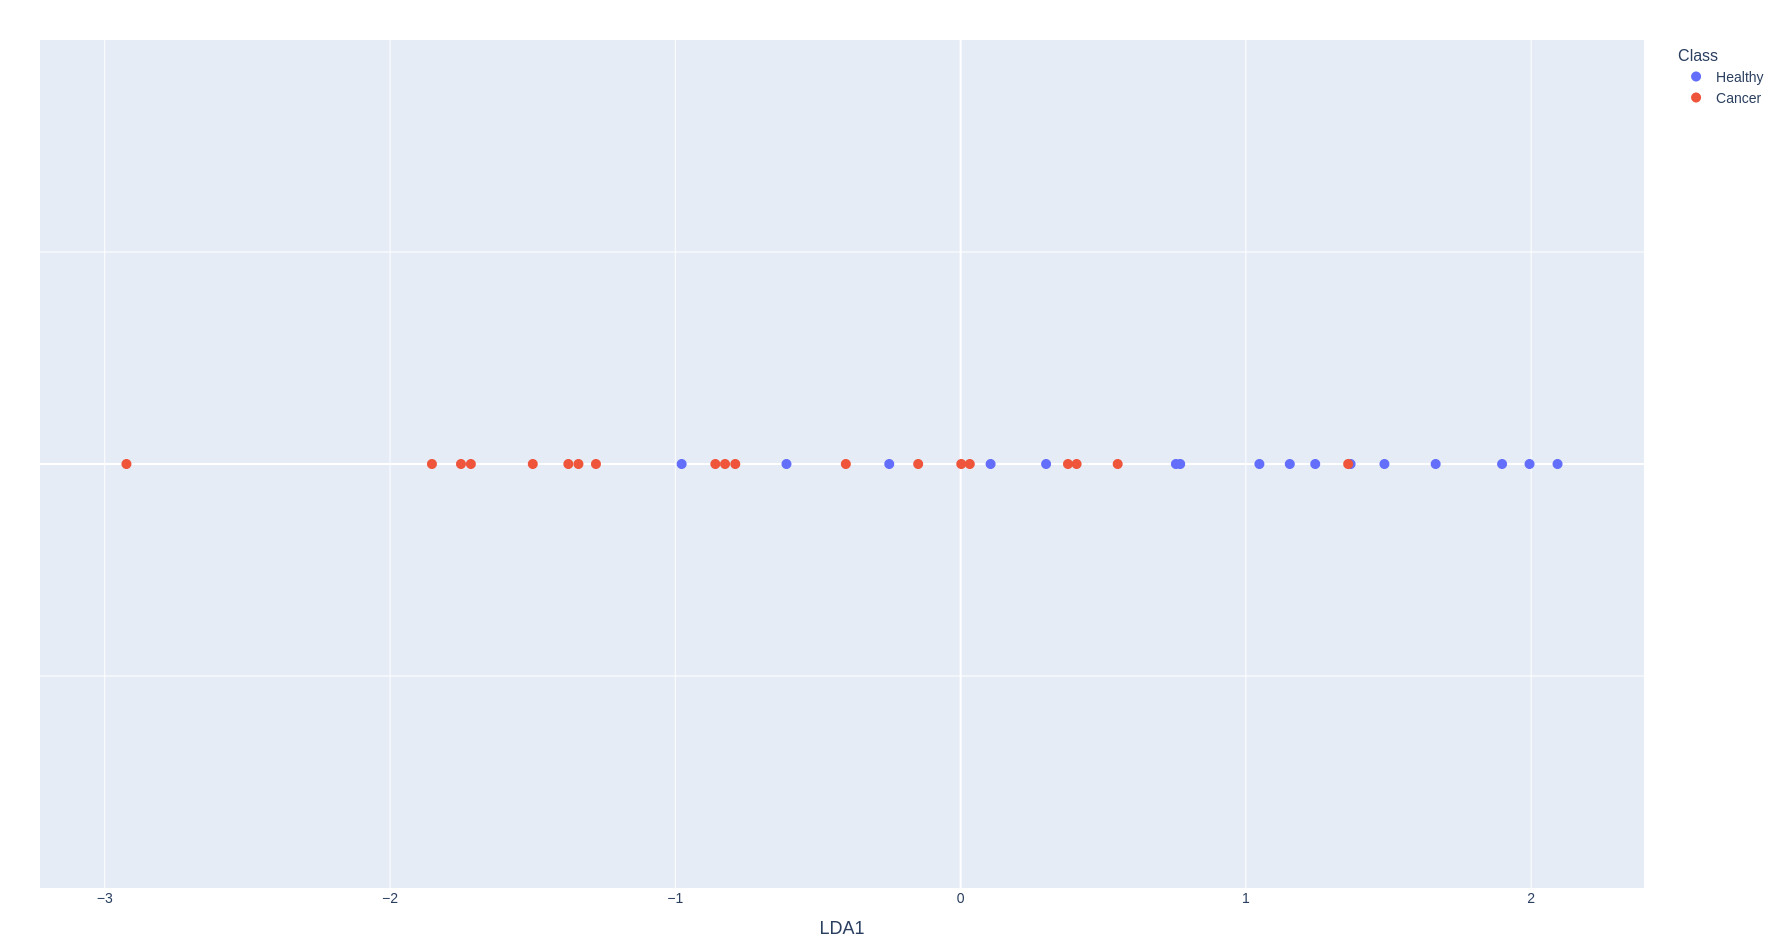
\includegraphics[width=1.1\textwidth]{images/LDA1.png}
    \caption{Linear Discriminant in one dimension.}
    \label{fig:ld1}
\end{figure}
\noindent
By applying the classifiers with the testing data projected in the LDA, the resulting performance metrics are presented in the table below.
=======
%\begin{figure}[H] 
%    \centering
%    \includegraphics[width=1.1\textwidth]{LD1.png}
%    \caption{PC1}
%    \label{fig:ld1}
%\end{figure}
>>>>>>> parent of b00b1e1 (commit final meta1)

\begin{table}[H]
\centering
\caption{Classifier results using the linear projection obtained by LDA (1D).}
<<<<<<< HEAD
\begin{tabular}{lcc}
\hline
\textbf{Metric} & \textbf{Euclidean} & \textbf{Mahalanobis} \\
\hline
Sensitivity (\%) & 78.9 & 78.9 \\
Specificity (\%) & 88.7 & 88.7 \\
Precision (\%) & 89.4 & 89.4 \\
F1-score (\%) & 83.7 & 83.7 \\
Accuracy (\%) & 83.4 & 83.4 \\
ROC-AUC (\%) & 90.9 & 91.8 \\
=======
\begin{tabular}{lccc}
\hline
\textbf{Metric} & \textbf{Euclidean} & \textbf{Mahalanobis} & \textbf{Fisher LDA} \\
\hline
Sensitivity (\%) & 84.21 & 84.21 & 84.21 \\
Specificity (\%) & 81.25 & 81.25 & 81.25 \\
Precision (\%) & 84.21 & 84.21 & 84.21 \\
F1-score (\%) & 84.21 & 84.21 & 84.21 \\
Accuracy (\%) & 82.86 & 82.86 & 82.86 \\
>>>>>>> parent of b00b1e1 (commit final meta1)
\hline
\end{tabular}
\label{tab:lda1d_classifiers}
\end{table}

<<<<<<< HEAD
Analyzing the values in Table \ref{tab:lda1d_classifiers}, a clear improvement can be observed across all performance metrics for all classifiers, as expected using a supervised approach. It is also worth noting that the Fisher LDA classifier was not applied to the LDA features, as explained in Section \ref{sec:lda_fisherlda}.

\subsection{Similarities between Mahalanobis and Fisher LDA classifiers}
\label{sec:mahalanobis_fisher}
\noindent
The identical results obtained with the Mahalanobis classifier and the Fisher LDA are theoretically expected, as both methods are mathematically equivalent under specific conditions. In the case of two-class classification problems, such as distinguishing Healthy from Cancer samples, and assuming that both classes follow approximately Gaussian distributions with equal covariance matrices, the Fisher LDA can be interpreted as a particular form of the Mahalanobis classifier. Both approaches rely on the same discriminant function, defined by a linear combination of features using the inverse of the within-class covariance matrix multiplied by the difference between the class mean vectors. Consequently, they define the same decision boundary in the feature space. In this dataset, these criteria are probably met, resulting in near identical results.

\subsection{Fisher LDA not applied to LDA}
\label{sec:lda_fisherlda}

\noindent
Applying the Fisher LDA classifier after performing LDA-based feature reduction is unnecessary because the dimensionality reduction step already computes the optimal linear discriminant directions used by Fisher’s method. The transformed feature space produced by LDA inherently encodes the maximum class separability, making any subsequent Fisher classification redundant and mathematically equivalent to the projection already achieved.

\section{Conclusion}

The comparative analysis of feature selection and dimensionality reduction methods demonstrated that the classification performance depends on the quality and relevance of the extracted features. The violin plots and ROC-AUC analysis revealed that Glucose, HOMA, Resistin, and Insulin exhibit higher discriminative power between Healthy and Cancer groups. Both ROC-AUC ranking and the Kruskal–Wallis test consistently identified these same features as the most informative, confirming their statistical significance and relevance for class separation.

When all features were used, the classifiers achieved moderate performance, with sensitivity and F1-score values below the desired threshold. After feature selection, slight improvements were observed, although the enhancement was not substantial, suggesting that redundant or weakly correlated features had limited impact on model performance. PCA-based dimensionality reduction, especially when retaining seven components that explained 95\% of the variance, led to a more compact representation while maintaining comparable classification results.

Among the classifiers, the Mahalanobis and Fisher LDA methods consistently produced identical results, as expected from their theoretical equivalence under equal covariance assumptions. Both outperformed the Euclidean classifier across all tests, highlighting the importance of incorporating covariance information in the classification process. The application of LDA for supervised dimensionality reduction proved particularly effective, as the resulting one-dimensional projection achieved the highest overall metrics, with clear improvement in accuracy, precision, and ROC-AUC.

Overall, the results indicate that supervised linear methods such as LDA, which exploit class label information, provide superior class separation compared to unsupervised approaches like PCA. These findings confirm that linear discriminant techniques can be effective for feature analysis, but not obtaining very good overall results.



=======
>>>>>>> parent of b00b1e1 (commit final meta1)
\end{document}

